\begin{enumerate}[label=\arabic*.,ref=\theenumi]
\numberwithin{equation}{enumi}
\item The op amp in the circuit of Fig. \ref{fig:ee18btech11028_2_q} has an open-loop gain of $10^{5}$ and a single-pole rolloff with $\omega_{3dB}$ = 10 rad/s.

\renewcommand{\thefigure}{\theenumi.\arabic{figure}}
%
\begin{figure}[!ht]
	\begin{center}
		\resizebox{\columnwidth}{!}{\input{./figs/ee18btech11028/question_fig.tex}}
	\end{center}
\caption{}
\label{fig:ee18btech11028_2_q}
\end{figure}
%
\begin{table}[!ht]
    \centering
    \input{./tables/ee18btech11028/ee18btech11028_2_t1.tex}
    \caption{}
    \label{table:ee18btech11028_2_parameters}
\end{table}

\item Sketch a Bode plot for the loop gain.
\\
\solution
Op-amp in our question has an open loop gain characterised by a single pole $P_{11} $ from table \ref{table:ee18btech11028_2_parameters} i.e.
\begin{align}
    G(s) = \frac{10^5}{1 + \frac{s}{P_{11}}}
        \label{eq:ee18btech11028_2_2}
\end{align}

Using voltage division on Fig. \ref{fig:ee18btech11028_2_q} we obtain,
\begin{align}
    H(s) = \frac{V_{f}}{V_{o}}
     &= \frac{\frac{1}{sC_{f}}}{R_{f} + \frac{1}{sC_{f}}}
    \\
    \implies H(s) = \frac{1}{1 + \frac{s}{P_{21}}}
        \label{eq:ee18btech11028_2_1}
\end{align}
where, 
\begin{align}
    P_{21} = \frac{1}{R_{f}C_{f}} = 1000
\end{align}

The loop gain is, 
\begin{align}
    GH(s) = \frac{10^5}{(1+\frac{s}{10})(1 + \frac{s}{1000})}
\end{align}

\begin{figure}[!ht]
    \centering
    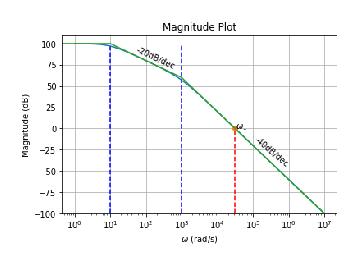
\includegraphics[width=\columnwidth]{./figs/ee18btech11028/ee18btech11028_2_1.eps}
    \caption{Magnitude plot}
    \label{fig:ee18btech11028_2_1}
\end{figure}


\begin{figure}[!ht]
    \centering
    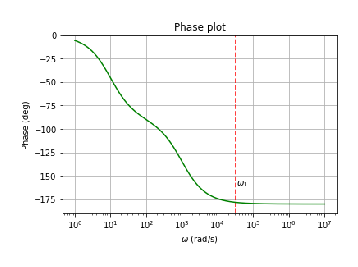
\includegraphics[width=\columnwidth]{./figs/ee18btech11028/ee18btech11028_2_2.eps}
    \caption{Phase plot}
    \label{fig:ee18btech11028_2_2}
\end{figure}


\item Find the frequency at which $ |GH|= 1$, and find the corresponding phase margin.
\\
\solution
Value of $\omega$ for unity magnitude can be obtained from Fig. \ref{fig:ee18btech11028_2_1} which is approximately $3 \times 10^{4}$.
More precise value can be obtained by solving for $\omega$ in,
\begin{align}
    \frac{10^{5}}{\sqrt{1 + \frac{w_{1}^{2}}{P_{1}^{2}}} \sqrt{1 + \frac{w_{1}^{2}}{P_{2}^{2}}}} = 1
\end{align}

Thus, 

\begin{align}
     \omega_{1} = 3.15 \times 10^{4} rad/s
\end{align}
The phase margin visibly from the Fig. \ref{fig:ee18btech11028_2_2} is very small.
\begin{align}
    PM = 180 \degree - \tan^{-1}(\frac{\omega_{1}}{10}) - \tan^{-1}(\frac{\omega_{1}}{1000})
      & = 1.84 \degree
\end{align}

\item Find the closed-loop transfer function, including its zero
and poles. Sketch a pole-zero plot. Sketch the magnitude of
the transfer function versus frequency, and label the important parameters on your sketch.
\\ 
\solution

\begin{align}
    T(s) = \frac{G(s)}{1 + G(s)H(s)}
    \\
\end{align}

From \eqref{eq:ee18btech11028_2_1} and \eqref{eq:ee18btech11028_2_2} we have,
\begin{align}
    \implies T(s) = \frac{10^{6}(s+1000)}{s^{2} + 1010s + 10^{4} + 10^{9}}
    \\
\end{align}

Zeros of closed loop transfer function,
\begin{align}
    Z_{1} = -1000
\end{align}

Similarly for poles,
\begin{align}
    s^{2} + 1010s + 10^{4} + 10^{9} = 0
    \\
    \implies P_{1}, P_{2} = -505 \pm j31618.9
\end{align}

\begin{figure}[!ht]
    \centering
    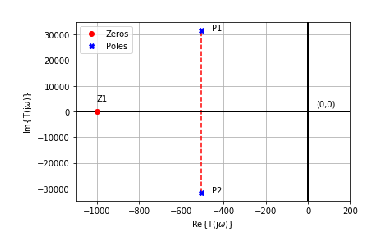
\includegraphics[width=\columnwidth]{./figs/ee18btech11028/ee18btech11028_2_3.eps}
    \caption{Pole zero plot}
    \label{fig:ee18btech11028_2_3}
\end{figure}


\begin{figure}[!ht]
    \centering
    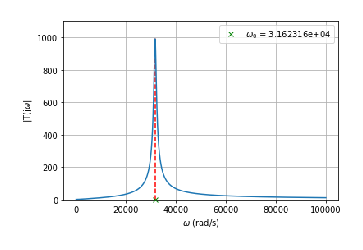
\includegraphics[width=\columnwidth]{./figs/ee18btech11028/ee18btech11028_2_4.eps}
    \caption{Closed loop magnitude plot}
    \label{fig:ee18btech11028_2_4}
\end{figure}

Poles are at $\omega_{0} = 3.16 \times 10^{4}$

\item The following python code plots  Fig. \ref{fig:ee18btech11028_2_1}, Fig. \ref{fig:ee18btech11028_2_2}, Fig. \ref{fig:ee18btech11028_2_3} and Fig. \ref{fig:ee18btech11028_2_4}.
\begin{lstlisting}
codes/ee18btech11028/ee18btech11028_2.py
\end{lstlisting}

\end{enumerate}